%\documentclass[12pt]{article}
%\usepackage{graphicx}
%\usepackage{graphics}
%\usepackage{refstyle}
%\usepackage{amsmath}
%\usepackage{caption}
%\usepackage{float}
%\usepackage{booktabs}
%\usepackage{array}
%\usepackage{amssymb}
%\usepackage{booktabs}
%\let\vec\mathbf
%\providecommand{\brak}[1]{\ensuremath{\left(#1\right)}}
%\graphicspath{{/storage/self/primary/Download/latexnew/fig}}                                     
$\vec{P}$ and $\vec{Q}$ are any two points lying on the sides $DC$ and $AD$ respectively of a parallelogram $ABCD$.Show that, $ar\brak{\triangle APB}=ar\brak{\triangle BQC}$.


\textbf{Figure:}
\begin{figure}[H]
    \centering
	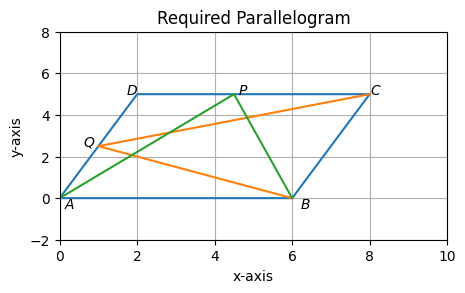
\includegraphics[width=\columnwidth]{chapters/vectors/exer/figs/1.png}
    \caption{}
    \label{fig:fig:1}
\end{figure}


\textbf{Solution:}
\begin{table}[H]
   \centering
  \begin{tabular}{|c|c|c|}
 \hline
    \textbf{Input Parameters} &\textbf{Description} &\textbf{Value} \\
    \hline
     $\vec{A}$& Vertex(at origin)&$\vec{0}$\\
     \hline
	$a$& Side of the parallelogram,$AB = DC$ & 6 \\
     \hline
	$b$& Side of the parallelogram,$AD = BC$ & $\sqrt{29}$\\
     \hline
	$\theta$&Angle of parallelogram,$\angle BAD$&$\sin^{-1}\brak{\frac{5}{\sqrt{29}}}$\\
     \hline
	$k_1$&$AQ:QD$&$k_1$\\
     \hline  
	$k_2$ & $DP:PC$ & $k_2$\\
     \hline  
\end{tabular}

   \caption{Table of input parameters}        
\label{tab:tab:1}                    
\end{table}




\begin{table}[H]
    \centering                                  
\begin{tabular}{|c|c|c|}
\hline
    \textbf{Output Parameters} &\textbf{Description} &\textbf{Value} \\
    \hline
     $\vec{B}$ &Vertex of parallelogram&$a\vec{e_1}$\\
      \hline
     $\vec{D}$ &Vertex of parallelogram &$b\begin{pmatrix} \cos{\theta}\\\sin{\theta}
     \end{pmatrix}$\\
     \hline
     $\vec{C}$&Vertex of parallelogram&$\vec{B}+\vec{D}$\\
     \hline
      $\vec{ Q}$ &Vertex of $\triangle BQC$&$\frac{k_1\vec{D}+\vec{A}}{k_1+1}$\\
     \hline
      $\vec{P}$ &Vertex of $\triangle APB$&$\frac{k_2\vec{C}+\vec{D}}{k_2+1}$\\
   \hline
\end{tabular}
                  
\caption{Table of output parameters}
\label{tab:tab:2}
 \end{table}


For the $\triangle BQC$, the vertices of the triangle are taken from \tabref{tab:tab:1} and \tabref{tab:tab:2}.

\begin{align}
\implies ar\brak{\triangle BQC}&=
\frac{1}{2}\begin{tabular}{|c c c|}            
1 &1&1\\                      
$\vec{B}$&$\vec{Q}$&$\vec{C}$\\    
\end{tabular}\\
&= \frac{1}{2}\begin{tabular}{|c c c|}
       1 &1&1\\
       6&$\frac{2k_1}{k_1+1}$&8 \\
       0&$\frac{5k_1}{k_1+1}$&5
   \end{tabular}\\
  \xrightarrow{C_2'=C_2-C_1,C_3'=C_3-C_1}&\frac{1}{2} \begin{tabular}{|c c c|}
       1 &0&0\\
       6&$\frac{-4k_1-6}{k_1+1}$&2 \\
       0&$\frac{5k_1}{k_1+1}$&5
   \end{tabular}\\
&=\frac{1}{2}\brak{1\begin{tabular}{|c c|}
   $\frac{-4k_1-6}{k_1+1}$ &2  \\
   $\frac{5k_1}{k_1+1}$ & 5
\end{tabular} +0+0}\\
&=\frac{1}{2} \times30\\                          
&=15 \end{align}


For the $\triangle APB$, the vertices of the triangle are taken from \tabref{tab:tab:1} and \tabref{tab:tab:2}.
   \begin{align}
  \implies ar\brak{\triangle APB} &=
\frac{1}{2}\begin{tabular}{|c c c|}            
1 &1&1\\                            
$\vec{A}$&$\vec{P}$&$\vec{B}$\\
\end{tabular}\\ &=  \frac{1}{2}
   \begin{tabular}{|c c c|}
       1 &1&1\\
       0&$\frac{8k_2+2}{k_2+1}$&6 \\
       0&5&0
   \end{tabular}\\
 &=\frac{1}{2} \times30\\
 &=15 \end{align}
 \brak{6} = \brak{10}


So, ar\brak{\triangle BQC} = ar\brak{\triangle APB}.\brak{proved}
%\end{document}


